
\setcounter{law}{1}

This series of lectures covers the fundamentals of thermodynamics. It begins with a treatment of the first law of thermodynamics and work. We then introduce the second law by the Kelvin-Planck and Clausius statements and relate these to the Carnot engine. Next, we discuss the second law of thermodynamics from the perspective of entropy, count microstates, and use Stirling's approximation to get interesting results from a statistical mechanics point of view. Finally, we derive Maxwell's relations of thermodynamic potentials, which are useful because they relate difficult-to-measure quantities to others than can be easily measured. 

\section{First Law and Work}
\subsection{Introduction}
Thermodynamics deals with the relations and transformations between heat and other forms of energy, especially mechanical work. Unlike classical mechanics, it considers macroscopic properties of systems consisting of many particles in which it is impractical to set up equations of motion for each individual particle. The first law of thermodynamics, which is discussed in this section, shows how work and heat relate through the conservation of energy. The laws of thermodynamics can be understood through a kinetic interpretation based on statistical mechanics, which describes the behavior of large ensembles of particles.
\subsection{Setup}
We describe our thermodynamics systems using the pressure $P$, volume $V$, and temperature $T$. These are average properties of the macroscopic systems, as we do not care about the motions of each individual particle but rather the macroscopic behavior. 

We characterize the geometry of the system purely using the volume. The majority of thermodynamical properties are independent of shape, so volume is the only geometric quantity given. For high surface area cases, this assumption breaks down - the surface area must also be considered.

Given a certain amount of the substance contained in a system, the volume, temperature, and pressure are not independent quantities. Instead, they are connected by an \textit{equation of state} of the form $$f(P,V,T) = 0.$$ This equation depends on the properties of the substance of which the systems consists. For example, for an ideal gas, the equation of state is the \textit{ideal gas law} $$PV = nRT.$$

We typically use PV diagrams to represent a thermodynamic system. Volume is on the horizontal axis and pressure is on the vertical, and a point on the plane defines the state of the system. Thermodynamic processes are represented by curves drawn between two points.

There are two main classes of transformations: \textit{reversible} and \textit{irreversible}. A reversible transformation takes place when the external conditions are changed so slowly that the system has time to adjust to equilibrium during each step of the transformation. Reversible transformations can, as the name suggests, be reversed by realizing the opposite sequence of steps. When the intermediate states are not states of equilibrium, the transformation is irreversible. 

During a transformation, we define $W$ to be the work done by the system on its surroundings. $W$ is positive if the system has performed work on its surroundings and negative if the surroundings have performed work on the system. We can relate this quantity to the internal variables of the system. We know that $dW = \vec{F}\cdot d\vec{r}.$ If we imagine expanding the system normal to its walls, we have $dV = A dr$ and $P = \tfrac{F}{A}$, so $dW = P dV$. In general, we then have that \begin{align}W &= \int\limits_{V_1}^{V_2} P dV.\label{eq:W} \end{align} This is the area beneath the curve connecting one state to another. If the curve is a loop, the work done is the area of the loop if the loop is traversed clockwise.

Finally, we define several special types of transformations. If volume is held constant, the process is \textit{isochoric}; if temperature is constant, it is \textit{isothermic}; if pressure is constant, it is \textit{isobaric}; and if no heat is transferred in or out of the system, it is \textit{adiabatic}.
\subsection{Ideal Gas Law}
We now derive the equation of state for an ideal gas. Consider a collection of ideal gas particles of mass $m$ and speed $v$ in a box, and assume the motion of these particles is random, meaning that the forces between the particles are negligible. Let there be $N$ particles in the system, and let the density of particles be $n = \tfrac{N}{V}$.

We now calculate the pressure on a side of the box with area $A$. Consider a particle with speed $v_x$ in the $x$-direction that collides elastically with the wall of the box. The particle reverses direction after the collision, so it imparts an impulse $2mv_x$ on the wall. In a time $\Delta t$, only particles close enough to the wall will deliver an impulse. These particles occupy a volume $A v_x \Delta t$, so the number of particles that hit the side of the box is $nAv_x \Delta t$. Then the force is $$F = 2mnAv_x^2,$$ so $$P = nmv_x^2.$$ 

The above expression assumes that all particles have the same velocity. However, as they all move in different directions, and only about half of them will be moving towards the side of the box, we have $$P = nm \left<v_x^2\right>.$$

Of course, we have three linearly independent directions in the volume, none of which is particularly unique. We assume therefore that $$\left<v_x^2\right> = \left<v_y^2\right> = \left<v_z^2\right> = \frac{1}{3} \left<v^2\right>,$$ where $\left<v^2\right>$ is the overall average squared velocity. Then $$PV = \frac{1}{3} nm \left<v^2 \right> V = \frac{2}{3} N \left<\frac{1}{2} mv^2\right> = \frac{2}{3} U,$$ where $U$ is the \textit{internal energy} of the system (that is, the kinetic energy of the particles within the system).

We note that, more generally, we define $K$ such that \begin{align}PV = (K-1) U.\label{eq:K}\end{align} As shown here, $K = \tfrac{5}{3}$ for a monatomic gas. 

Intuitively, the internal energy $U$ is proportional to the temperature $T$. We can show that they must be proportional at an equilibrium between two systems. From experiment, we are aware that two systems at different temperatures that can transfer heat to each other will eventually settle down to have the same temperature. We may argue that the same is true of internal energy. Suppose these two systems were in contact with each other and separated by a sliding boundary. We may argue that the velocity of the boundary can be modeled as the velocity of the center of mass of a new system of a particle from each system colliding with each other with the average velocities of particles in the two systems. In this case, since energy and momentum are conserved, the momenta of these particles simply change direction. At equilibrium, where the boundary does not move, it must then be true that the particles must have the same kinetic energy, as the energy is conserved. This establishes that the average kinetic energy is proportional to the temperature at an equilibrium between two systems. We then define $k$ such that $\left<KE\right> = \frac{3}{2}kT$. In this case, $k$ is called the \textit{Boltzmann constant}. This gives $$U = \frac{3}{2}NkT$$

Plugging this in to our earlier derived expression, we have that $$PV =NkT,$$ and if we wish to express this in terms of moles of gas, defining the ideal gas constant $R$ to be $k \cdot N_A$, where $N_A$ is Avogadro's constant, we have the familiar \begin{align}PV &= nRT,\label{eq:id}\end{align}
where $n$ is the number of moles of gas, usually taken to be 1. A similar substitution (assuming $n = 1$) also gives us that, for an ideal gas, \begin{align}U &= \frac{3}{2} RT.\label{eq:U}\end{align} Equations \ref{eq:id} and \ref{eq:U} will be useful for problems involving ideal gases. 


\subsection{First Law of Thermodynamics}
The first law of thermodynamics is a statement of the conservation of energy. It states that any change in the internal energy of the system must be caused by a change in heat or work done by the system: $$dU = -\delta W + \delta Q.$$ Note that $W$ is negative here because it is the work done \textit{by the system on the surroundings}. We use the $\delta$s to denote that these quantities are path-dependent on a PV diagram.

We now define the heat capacity, or thermal capacity, of system as $$C = \frac{\delta Q}{dT}.$$  There are different heat capacities at constant volume and pressure.

At constant volume, we write $U$ as a function of $V$ and $T$ (recalling that $T$, $P$, and $V$ are not independent), so $U = U(T,V)$. Then $$dU = \left(\frac{\partial U}{\partial V}  \right)_T dV + \left(\frac{\partial U}{\partial T}  \right)_V dT =\left(\frac{\partial U}{\partial T}  \right)_V dT .$$ The first law gives $$\delta Q = dU + P dV =\left(\frac{\partial U}{\partial T}  \right)_V dT,$$ so $$C_V = \frac{\delta Q}{dT} = \left(\frac{\partial U}{\partial T}  \right)_V.$$

When pressure is held constant, we instead write $U = U(P,T).$ Then  $$dU = \left(\frac{\partial U}{\partial P}  \right)_T dP + \left(\frac{\partial U}{\partial T}  \right)_P dT =\left(\frac{\partial U}{\partial T}  \right)_P dT .$$ By the first law,
$$\delta Q = dU + P dV = dU + P\left[\left(\frac{\partial V}{\partial T} \right)_P dT+\left(\frac{\partial V}{\partial P} \right)_T dP \right] = \left[\left(\frac{\partial U}{\partial T}  \right)_P + P \left(\frac{\partial V}{\partial T} \right)_P \right] dT$$ so $$C_P = \frac{\delta Q}{dT} = \left(\frac{\partial U}{\partial T}  \right)_P+P\left(\frac{\partial V}{\partial T} \right)_P.$$ 

For an ideal gas, $$\left(\frac{\partial U}{\partial T}  \right)_P=\left(\frac{\partial U}{\partial T}  \right)_V = \frac{dU}{dT},$$ so $$C_P = C_V + P\left(\frac{\partial V}{\partial T} \right)_P = C_V + R.$$ We find also that $$K-1 = \frac{R}{C_V},$$ where $K$ is defined in equation \ref{eq:K}.

With this background, we can now consider ideal gases undergoing adiabatic transformations. We specifically study these because the other transformations are comparatively easy to analyze. Adiabatic transformations have $\delta Q = 0$, so \begin{align*} C_V dT &= -P dV, \\ C_V dT &= - \frac{RT}{V} dV, \\ \frac{dT}{T} &= \frac{R}{C_V} \frac{dV}{V} .\end{align*} Integrating both sides, we have $$\ln \left(\tfrac{T}{T_0} \right) = \frac{R}{C_V} \ln \left(\tfrac{V}{V_0} \right).$$ This means that \begin{align} TV^{K-1} &= PV^K = D \label{eq:ad}\end{align}for some constant $D$ during adiabatic transformations for ideal gases. For monatomic gases, equation \ref{eq:ad} implies that $PV^{\tfrac{5}{3}}$ is constant during adiabatic transformations. 
\section {Carnot Cycle and Second Law}
\subsection{Statements of the Second Law of Thermodynamics}
These are two equivalent statements of the second law of thermodynamics.
\begin{quote}
\textbf{Kelvin-Planck Statement}: No system can absorb heat from a single reservoir and convert it entirely into work without additional net changes in the system or its surroundings.
\end{quote}
\begin{quote}
 \textbf{Clausius Statement}: A process whose only net result is to absorb heat from a cold reservoir and release the same amount of heat to a hot reservoir is impossible.
\end{quote}
 
We can show that the Kelvin-Planck and Clausius statements are equivalent by proving that, if either of these postulates is false, the other is also false. In particular, let us first assume that the Kelvin-Planck statement is false. Then we could perform a transformation whose sole result is to transform a definite amount of heat from a source at temperature $T_1$ to work. By means of friction, we could convert this work back to heat, thus raising the temperature of another body regardless of the value of its initial temperature $T_2$. If we let $T_2 > T_1$, the result of this transformation would be the transfer of heat from a cold reservoir to a hot reservoir without any loss, in violation of the Clausius statement. To show that the Kelvin-Planck statement must be false when the Clausius statement is false, we must discuss heat engines, particularly the Carnot cycle. 
\subsection{The Carnot Cycle}
The Carnot cycle is the particular heat engine shown in figure \ref{fig:carnot}. It consists of four reversible steps:
\begin{enumerate}
\item Isothermal absorption of heat from a hot reservoir,
\item Adiabatic expansion to a lower temperature,
\item Isothermal release of heat into a cold reservoir,
\item Adiabatic compression to the original state.
\end{enumerate}

\begin{figure}[ht]
\centering
\caption{Carnot Cycle}
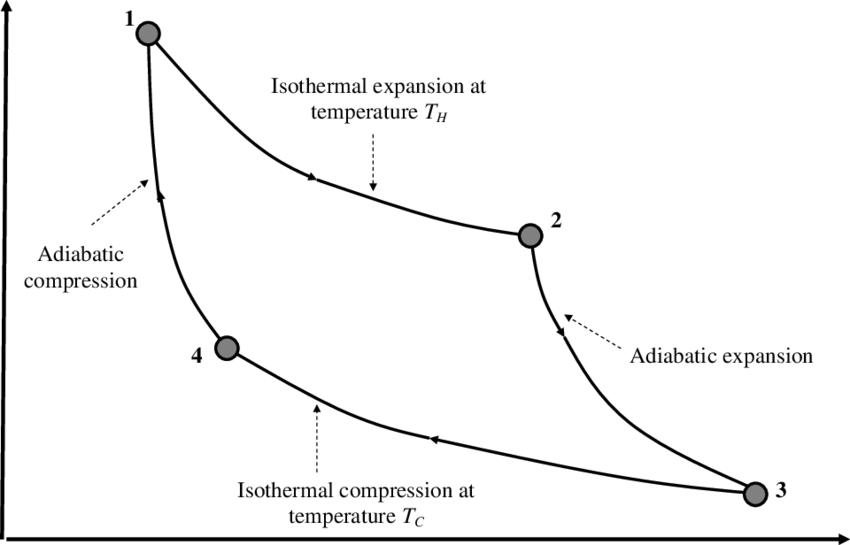
\includegraphics[width=8cm]{images/thermo/carnot.png}
\label {fig:carnot}
\end{figure}

By the first law, the work done by this heat engine on its surroundings is equal to the net heat gained by the system. Let $Q_H$ be the heat gained during step 1 and $Q_C$ be the heat released in step 4. Then the work done is $Q_H - Q_C$, and the efficiency is $$\eta = \frac{Q_H-Q_C}{Q_H} = 1-\frac{Q_C}{Q_H}.$$

We can calculate $Q_H$ as $$Q_H = W_{\text{by gas}} = \int \limits_{V_1}^{V_2} P dV = \int  \limits_{V_1}^{V_2} \frac{n R T_H}{V} dV = nR T_H \ln \left(\frac{V_2}{V_1}\right).$$ Similarly, we have $$Q_C = W_{\text{on gas}} = nRT_C \ln \left(\frac{V_3}{V_4}\right).$$

From the rule we derived early for adiabatic processes, we have 
\begin{align*}
T_H V_2^{K-1} &= T_C V_3^{K-1},\\ 
T_H V_1^{K-1} &= T_C V_4^{K-1},
\end{align*}
so 
$$\frac{V_2}{V_1} = \frac{V_3}{V_4}.$$

Thus, the heat ratio is
\begin{align*}
\frac{Q_C}{Q_H} &= \frac{T_C}{T_H}, 
\end{align*} 
so the efficiency is \begin{align}\eta &=1-\frac{T_C}{T_H}. \label{eff} \end{align}

We can now prove that the Kelvin-Planck statement must be false when the Clausius statement is false. Assume that we can transfer heat $Q_H$ from the reservoir at $T_C$ to $T_H$ with no other effects. We can then run the Carnot cycle and deliver heat $Q_C$ to the reservoir at $T_C$ and perform some work. The end result is that there was no net heat change at the reservoir at $T_H$, the reservoir at $T_C$ had some heat loss, and work was performed. This violates the Kelvin-Planck statement, as we have extracted heat from the reservoir at $T_C$ and converted it to work without any other effects. 

\subsection{Carnot's Theorem}
It turns out the Carnot cycle has the maximum possible efficiency of any heat engine. To prove this, consider the system in figure \ref{fig:proof}, where $\eta$ is the efficiency of the heat engine and $\eta'$ is the efficiency of the Carnot engine. The Carnot engine is run in reverse, as shown, and $T_1 > T_2$. If we have $\eta > \eta'$, the result is that heat is transferred from a cold reservoir to a hot one with no side effects. This directly violates the Clausius statement of the second law.

\begin{figure}[ht]
\centering
\caption{System for Carnot's Theorem Proof}
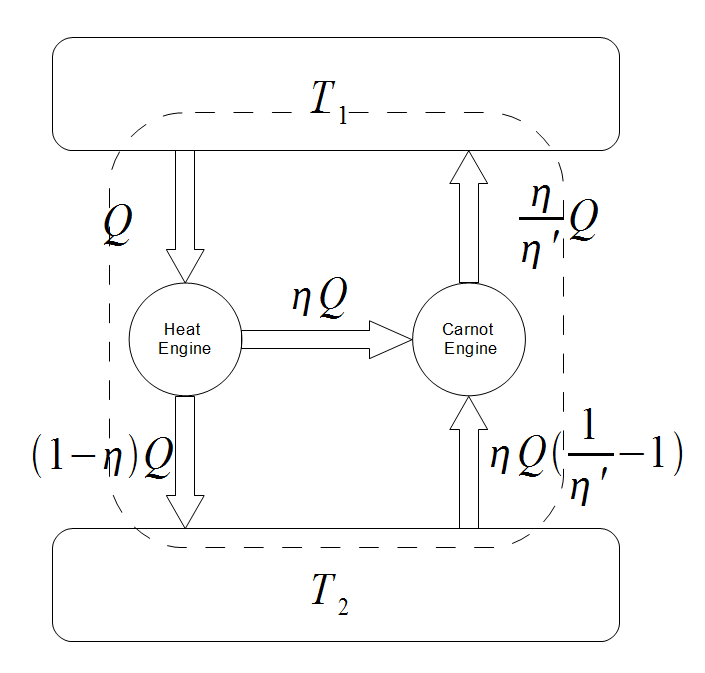
\includegraphics[width=6cm]{images/thermo/proof.png}
\label {fig:proof}
\end{figure}
\subsection{Entropy}
For our Carnot engine, we have $$\frac{Q_H}{T_H} = \frac{Q_C}{T_C}.$$ This means that the path integral of $\tfrac{\Delta Q}{T}$ is zero around our cycle. Based on this, we define the \textit{entropy} $S$ by the equation  $$\Delta S = \frac{\Delta Q}{T}.$$ Then $\Delta S = 0$ for the Carnot cycle (or any reversible transformation) and $\Delta S \geq 0$ in general.
\section {Entropy}
\subsection{The Second Law of Thermodynamics}
Recall that if the First Law of Thermodynamics is essentially a statement about what \textit{can} happen in a thermodynamical system, addressing energy and its conservation, then the Second Law is the one that dictates what will happen. We can think of the Second Law of Thermodynamics as giving a direction to time, philosophically, as it distinguishes processes that can happen while time progresses. The law itself can be phrased in a multitude of different ways, two of which are Clausius' and Kelvin's Postulates. Today, we'll phrase it differently: 
\begin{law}[The Second Law of Thermodynamics]
In a physical system, the \textit{entropy} $S$ of the system is non-decreasing, approaching a maximum value. 
\end{law}
We will be focused mostly on the nature of \textit{entropy}, our final state variable. Recall that a \textit{state variable} is one that only depends on the current configuration of particles in a system, and not on how the configuration was generated.

\subsection{Entropy and Statistical Mechanics}
To investigate entropy from a statistical mechanics perspective, we appeal to one of Boltzmann's results. First, define $\Omega$ to be the number of ways a state can be achieved/populated by the particles in the system. That is, given the energy distribution of the particles, $\Omega$ is the number of ways the atoms can be arranged to satisfy the conditions of the system. Boltzmann defines the entropy $S$ as 
\[
	S = k_B \ln \Omega,
\]
where $k_B$ is the \textit{Boltzmann constant}.
This allows one to derive the Third Law of Thermodynamics, where when we have one state ($\Omega = 1$) in a crystal lattice, the entropy of the system is zero. Not super relevant or particularly useful, but it's an interesting little corollary. 

We will now work in a \textit{micro-canonical ensemble}, where we fix the number of atoms $N$, the total energy of the system $E$, and the number of atoms in each of the $r$ energy states $n_k$, each associated with energy $\eps_k$. In variables, we have the following two constraints on our system: 
\[
	N = \sum_{k=1}^r n_k \quad E = \sum_{k=1}^r \eps_k n_k
\]
In general, in statistical mechanics (while working in equilibrium states), the micro-canonical ensemble is one of three main models used to describe a thermodynamical system. The others are the \textit{grand canonical ensemble} and the \textit{}
We can compute $\Omega$ and the entropy $S$ explicitly now: 
\[
	\Omega = \frac{N!}{n_1! n_2! \ldots n_r!} \implies S = k_B \ln \Omega = k_B \ln N! - k_B \sum_{k=1}^r \ln n_k!
\]
To maximize $S$, we have to use\ldots Lagrange multipliers! Consider the Lagrangian function
\[
	\lagr = S + \lambda\left(N - \sum_{k=1}^r n_k \right) + \mu \left(E - \sum_{k=1}^r \eps_k n_k\right) 
\]
and plugging in, we get 
\[
	\lagr = k_B \ln N! - k_B \sum_{k=1}^r \ln n_k! + \lambda\left(N - \sum_{k=1}^r n_k \right) + \mu \left(E - \sum_{k=1}^r \eps_k n_k\right) 
\]
We now compute $\pdv{\lagr}{n_j}$ and set it equal to 0: 
\[
	\pdv{\lagr}{n_j} = -k_B \pdv{}{n_j} \ln n_j! - \lambda - \mu \eps_j = 0
\]
So far, we've let the $n_i$s be integers, but in order to differentiate with respect to an $n_i$, we have to differentiate a factorial function. Since we're physicists, we're allowed to approximate, and so we can use \textit{Stirling's approximation}: 
\[
	n! \approx \left(\frac{n}{e}\right)^n \sqrt{2 \pi n} \implies \ln n! \approx n \ln n - n + \frac{1}{2} \ln 2\pi + \frac{1}{2} \ln n
\]
We're allowed to use this approximation that gets much better as $n_i$ gets very large (as we want them to be, usually), and so we can ``differentiate" $\ln n!$: 
\[
	\pdv{}{n} \ln n! \approx \ln n + 1 - 1 + \frac{1}{2n} \approx \ln n
\]
This gives us 
\[
	\pdv{\lagr}{n_j} = -k_B \ln n_j - \lambda - \mu \eps_j = 0
\]
If we pick different $n_j$, $n_k$, and we subtract them from each other, we have: 
\[
	\pdv{\lagr}{n_j} - \pdv{\lagr}{n_k} = -k_B \ln \frac{n_j}{n_k} - \mu (\eps_j - \eps_k) = 0 \implies k_B \ln n_j + \mu \eps_j = k_B \ln n_k + \mu \eps_k 
\]
Out of nowhere, we've found the invariant $k_B \ln n_k + \mu \eps_k$! With some foresight, let's let this constant be $k_B \ln A$: 
\[
	 k_B \ln n_k + \mu \eps_k = k_B \ln A \implies \ln \frac{n_k}{A} = -\frac{\mu \eps_k}{k_B} \implies n_k = A e^{-\frac{\mu \eps_k}{k_B}}
\]
This means the number of particles occupying state $k$ with energy $\eps_k$ is proportional to $e^{-\frac{\mu \eps_k}{k_B}}$ in equilibrium, derived from the fact that the entropy has to be maximized by the system. All we have to do now is to figure out what exactly $\mu$ is. 

The way we figure out what $\mu$ is by considering what happens what happens to the entropy $S$ when we move an atom from state $i$ to $j$. 
\begin{align*}
	dS &= k_B \ln \frac{N!}{n_1! n_2! \ldots (n_i-1)! \ldots (n_j+1)! \ldots n_r!} - k_B \ln \frac{N!}{n_1! n_2! \ldots n_i! \ldots n_j! \ldots n_r!} \\
	&= k_B \ln \frac{n_i}{n_j +1} \approx k_B \ln \frac{n_i}{n_j} = k_B \ln e^{\frac{\mu}{k_B}(\eps_j - \eps_i)} = \mu (\eps_j - \eps_i)
\end{align*}
This means that the change in entropy is directly proportional to the change in energy that the atom experiences, which is also the infinitesimal change in heat $\delta Q$! Assuming the process is reversible, we have $dS = \mu \delta Q$. We can make the final leap to claim that $\mu = \frac{1}{T}$, if we believe our definition of entropy from looking at Carnot cycles and heat engines.

This directly gives the most important thermodynamic fact in reversible processes, by way of the First Law of Thermodynamics: 
\begin{theorem}
The change in the internal energy $U$ is given by $dU = T dS - p dV$.
\label{thm-first}
\end{theorem}
This is a cool fact to tinker with and one can get all sorts of interesting relations amongst the state variables $p, V, T,$ and $S$. 

From this statistical perspective, entropy can be seen to be a measure of the ``disorder" of a system - the more ways a system can be populated, the higher the $\Omega$, and the higher the entropy. This can be interpreted (poorly) as the amount of ``chaos" present in the system, which is not a very useful way to think about the entropy. 

With this analysis of entropy, what we've also found is this underlying probability distribution of atoms occupying energy states, proportional to $e^{-\frac{\eps}{k_B T}}$, where $\eps$ is the energy of the state. This gives us an interesting probability distribution for ideal gases and how fast the atoms within them are moving. If we recall that the energy of a particle is $\frac{1}{2} mv^2$, where $v$ is the velocity, the probability distribution we have is now proportional to $e^{-\frac{mv^2}{2 k_B T}}$, normalized by some constant., which turns out to be
\[
    P(\vec v, d\vec v) = \left(\frac{m}{2\pi k_B T} \right)^{\frac{3}{2}} e^{-\frac{mv^2}{2 k_B T}}
\]
However, if we want to be working with a speed distribution, in our phase space, we have to ``integrate" this velocity distribution over all spheres of constant speed $v$, which gives us an extra term: 
\[
    P(v, dv) = \left(\frac{m}{2\pi k_B T} \right)^{\frac{3}{2}} 4\pi v^2 e^{-\frac{mv^2}{2 k_B T}}
\]
This gives us the \textit{Maxwell-Boltzmann speed distribution} for ideal gases, which is fairly accurate in real life and also gives us the energy for ideal gases as $U = \frac{3}{2} k_B T$, interestingly enough.

\section {Maxwell Relations}
\subsection{Introduction} In this lecture, we derive Maxwell's relations of thermodynamic potentials. These are useful because they relate difficult-to-measure quantities to others than can be easily measured. 
\subsection{Thermodynamic Potentials}
A \textit{thermodynamic potential} is a quantity used to represent some thermodynamic state in a system. Each thermodynamic potential represents a different ``type" of energy that the system has. There are \textit{natural variables} for each thermodynamic potential. When these variables are held constant, the associated potential is conserved.
\subsubsection{Internal Energy}
One example of a thermodynamic potential is \textit{internal energy}, which, as we know, is the energy of the system due to the motion of its constituent particles. Based on Theorem \ref{thm-first}, $U$ is conserved when $S$ and $V$ are both constant. Therefore, entropy and volume are the natural variables of internal energy. 
\subsubsection{Enthalpy}
The \textit{enthalpy} $H$ is another thermodynamic potential defined as $$ H = U + PV.$$ The enthalpy is the total heat content of the system - it measures the capacity to do non-mechanical or release heat.
 
We can derive $dH$ as follows. We have
\begin{align}
dH &= dU + P dV + V dP 
= TdS + VdP. \label{eq:H}
\end{align} 
Based on equation \ref{eq:H}, we can conclude that entropy and pressure are the natural variables of enthalpy.
\subsection{Helmholtz Free Energy}
Another thermodynamic potential is the \textit{Helmholtz free energy} $$F = U-TS.$$ This is the capacity to do useful work of any kind (mechanical and non-mechanical).

The differential form is 
\begin{align}
dF &= dU - TdS - SdT
= -PdV-SdT. \label{eq:F}
\end{align}
From equation \ref{eq:F}, we see that the natural variables of the Helmholtx free energy are volume and temperature.
\subsubsection{Gibbs Free Energy}
The final thermodynamic potential we will consider is the Gibbs free energy $$G = H-TS.$$ This measures how much non-mechanical work the system could do. We find that the differential form is 
\begin{align}
dG &= dH - TdS - S dT
= VdP - S dT \label{eq:G},
\end{align} 
so the natural variables of the Gibbs free energy are pressure and temperature.
\subsection{Derivation of Maxwell Relations}
\subsubsection{Internal Energy}
We write the internal energy $U$ as a function of its natural variables, $S$ and $V$, so the total differential is
$$dU = \left(\frac{\partial U}{\partial S} \right)_V dS + \left(\frac{\partial U}{\partial V} \right)_S dV.$$ Equating this to the differential form from Theorem \ref{thm-first} gives $$\left(\frac{\partial U}{\partial S} \right)_V dS + \left(\frac{\partial U}{\partial V} \right)_S dV = TdS - PdV,$$ so
\begin{align*}
\left(\frac{\partial U}{\partial V} \right)_S &= -P,\\
\left(\frac{\partial U}{\partial S} \right)_V &= T.
\end{align*}
Then we have
\begin{align*}
\left(\frac{\partial }{\partial S} \right)_V\left(\frac{\partial U}{\partial V} \right)_S &= -\left(\frac{\partial P }{\partial S} \right)_V,\\
\left(\frac{\partial }{\partial V} \right)_S\left(\frac{\partial U}{\partial S} \right)_V &= \left(\frac{\partial T}{\partial V} \right)_S.
\end{align*}
By Clairaut, we conclude that 
\begin{align}
 -\left(\frac{\partial P }{\partial S} \right)_V &= \left(\frac{\partial T}{\partial V} \right)_S \label{eq:m1}.
\end{align}
Equation \ref{eq:m1} is our first Maxwell relation.
\subsubsection{Enthalpy}
We use the same logic to derive the second Maxwell relation. Consider the enthalpy as a function of its natural variables, so that $H = H(S,P)$. Then we have 
$$dH = \left(\frac{\partial H}{\partial S} \right)_P dS + \left(\frac{\partial H}{\partial P} \right)_S dP = TdS+VdP,$$
so 
\begin{align*}
 \left(\frac{\partial H}{\partial S} \right)_P &= T, \\
  \left(\frac{\partial H}{\partial P} \right)_S &= V.
\end{align*}
Then 
\begin{align*}
\left(\frac{\partial }{\partial P} \right)_S\left(\frac{\partial H}{\partial S} \right)_P &= \left(\frac{\partial T }{\partial P} \right)_S,\\
\left(\frac{\partial }{\partial S} \right)_P\left(\frac{\partial H}{\partial P} \right)_S &= \left(\frac{\partial V }{\partial S} \right)_P,\\
\end{align*}
so 
\begin{align}
 \left(\frac{\partial T }{\partial P} \right)_S &= \left(\frac{\partial V }{\partial S} \right)_P \label{eq:m2}.
\end{align}
This is the second Maxwell relation.
\subsubsection{Helmholtz Free Energy}
We now consider the Helmholtz free energy as a function of its natural variables, so that $F = F(V,T)$. Then we have 
$$dF = \left(\frac{\partial F}{\partial V} \right)_T dV + \left(\frac{\partial F}{\partial T} \right)_V dT = -PdV-SdT,$$
so 
\begin{align*}
 \left(\frac{\partial F}{\partial V} \right)_T &= -P, \\
  \left(\frac{\partial F}{\partial T} \right)_V &= -S.
\end{align*}
Then 
$$ -\left(\frac{\partial P}{\partial T} \right)_V =
 \left(\frac{\partial }{\partial T} \right)_V\left(\frac{\partial F}{\partial V} \right)_T  = \left(\frac{\partial }{\partial V} \right)_T \left(\frac{\partial F}{\partial T} \right)_V = -\left(\frac{\partial S}{\partial V} \right)_T,
$$ so 
\begin{align}
 \left(\frac{\partial P }{\partial T} \right)_V &= \left(\frac{\partial S }{\partial V} \right)_T\label{eq:m3}.
\end{align}
This is the third Maxwell relation.
\subsubsection{Gibbs Free Energy}
Finally, we consider the Gibbs free energy as a function of its natural variables, so that $G = G(P,T)$. Then we have 
$$dG = \left(\frac{\partial G}{\partial P} \right)_T dP + \left(\frac{\partial G}{\partial T} \right)_P dT = V dP - S dT,$$
so 
\begin{align*}
 \left(\frac{\partial G}{\partial P} \right)_T &= V, \\
  \left(\frac{\partial G}{\partial T} \right)_P &= -S.
\end{align*}
Then 
$$ \left(\frac{\partial V}{\partial T} \right)_P =
 \left(\frac{\partial }{\partial T} \right)_P\left(\frac{\partial G}{\partial P} \right)_T  = \left(\frac{\partial }{\partial P} \right)_T \left(\frac{\partial G}{\partial T} \right)_P = -\left(\frac{\partial S}{\partial P} \right)_T,
$$ so 
\begin{align}
 \left(\frac{\partial V }{\partial T} \right)_P &= -\left(\frac{\partial S }{\partial P} \right)_T \label{eq:m4}.
\end{align}
This is the last Maxwell relation.
\subsection{Summary of Maxwell Relations}
We have derived the following Maxwell relations.
\begin{align*}
 -\left(\frac{\partial P }{\partial S} \right)_V &= \left(\frac{\partial T}{\partial V} \right)_S\\
\left(\frac{\partial T }{\partial P} \right)_S &= \left(\frac{\partial V }{\partial S} \right)_P\\
 \left(\frac{\partial P }{\partial T} \right)_V &= \left(\frac{\partial S }{\partial V} \right)_T\\
\left(\frac{\partial V }{\partial T} \right)_P &= -\left(\frac{\partial S }{\partial P} \right)_T
\end{align*}
These equations are useful because they relate difficult to measure quantities like $\left(\frac{\partial S }{\partial P} \right)_T$ to more easily measurable quantities like $\left(\frac{\partial V }{\partial T} \right)_P$. Note that they are not the only Maxwell relations; others can be derived for different thermodynamic potentials. 